\documentclass{article}%
\usepackage[T1]{fontenc}%
\usepackage[utf8]{inputenc}%
\usepackage{lmodern}%
\usepackage{textcomp}%
\usepackage{lastpage}%
\usepackage{graphicx}%
%
\title{Report created by ... Library on '43903' dataset}%
%
\begin{document}%
\normalsize%
\maketitle%
\section{Exploratory Data Analysis Part}%
\label{sec:ExploratoryDataAnalysisPart}%
\subsection{DataTypes and Non{-}Null Count}%
\label{subsec:DataTypesandNon{-}NullCount}%
Information is in table 1%


\begin{table}[h!]%
\caption{Dataset Columns Information}%
\vspace{0.2cm}%
\centering%
\begin{tabular}{|c|c|c|}%
\hline%
Column&Non{-}Null Count&Dtype\\%
\hline%
race&101766&object\\%
gender&101766&object\\%
age&101766&object\\%
admission\_source\_id&101766&object\\%
time\_in\_hospital&101766&uint8\\%
medical\_specialty&101766&object\\%
num\_lab\_procedures&101766&uint8\\%
num\_procedures&101766&uint8\\%
num\_medications&101766&uint8\\%
primary\_diagnosis&101766&object\\%
number\_diagnoses&101766&uint8\\%
max\_glu\_serum&101766&object\\%
A1Cresult&101766&object\\%
insulin&101766&object\\%
change&101766&object\\%
diabetesMed&101766&object\\%
medicare&101766&bool\\%
medicaid&101766&bool\\%
had\_emergency&101766&bool\\%
had\_inpatient\_days&101766&bool\\%
had\_outpatient\_days&101766&bool\\%
target&101766&int64\\%
\hline%
\end{tabular}%
\end{table}

%
\newpage%
\subsection{Descriptive Statistics}%
\label{subsec:DescriptiveStatistics}%
Information is in table 2%


\begin{table}[h!]%
\caption{Dataset Descriptive Statistics}%
\vspace{0.2cm}%
\centering%
\begin{tabular}{|c|c|c|c|c|c|c|c|c|}%
\hline%
Statistic&count&mean&std&min&25\%&50\%&75\%&max\\%
\hline%
time\_in\_hospital&101766.0&4.4&2.99&1.0&2.0&4.0&6.0&14.0\\%
num\_lab\_procedures&101766.0&43.1&19.67&1.0&31.0&44.0&57.0&132.0\\%
num\_procedures&101766.0&1.34&1.71&0.0&0.0&1.0&2.0&6.0\\%
num\_medications&101766.0&16.02&8.13&1.0&10.0&15.0&20.0&81.0\\%
number\_diagnoses&101766.0&7.42&1.93&1.0&6.0&8.0&9.0&16.0\\%
target&101766.0&0.11&0.31&0.0&0.0&0.0&0.0&1.0\\%
\hline%
\end{tabular}%
\end{table}

%
\newpage%
\subsection{Bar Charts for Categorical Columns and Histograms for Numerical Columns}%
\label{subsec:BarChartsforCategoricalColumnsandHistogramsforNumericalColumns}%


\begin{figure}[h!]%
\centering%
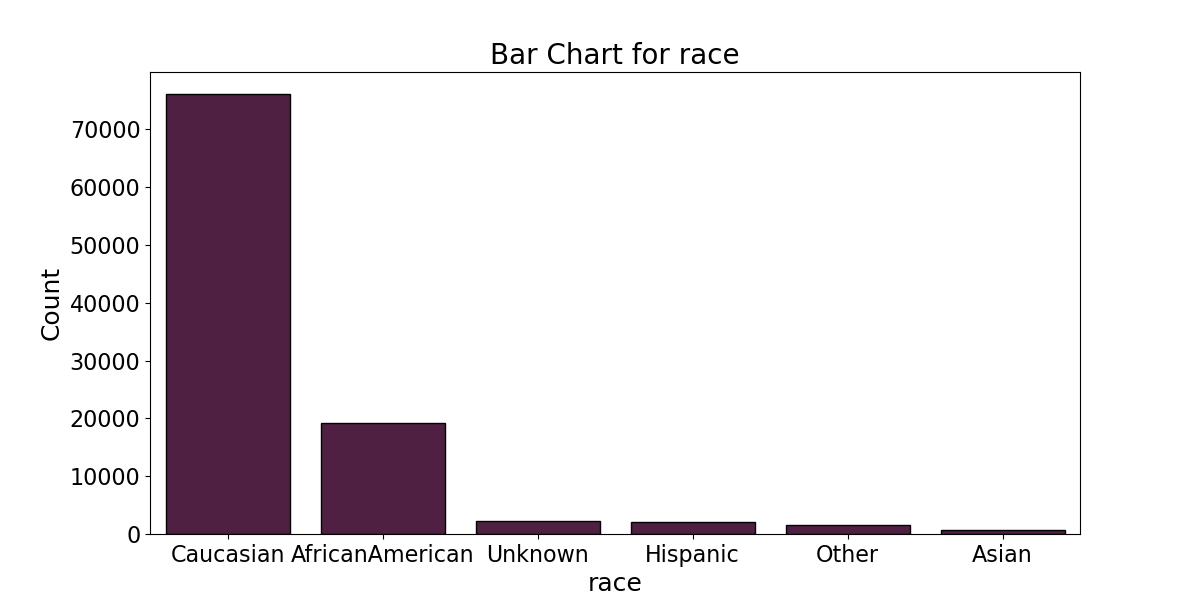
\includegraphics[width=200px]{eda/bar_charts/race_bar_chart.png}%
\caption{Bar Chart of race}%
\end{figure}

%


\begin{figure}[h!]%
\centering%
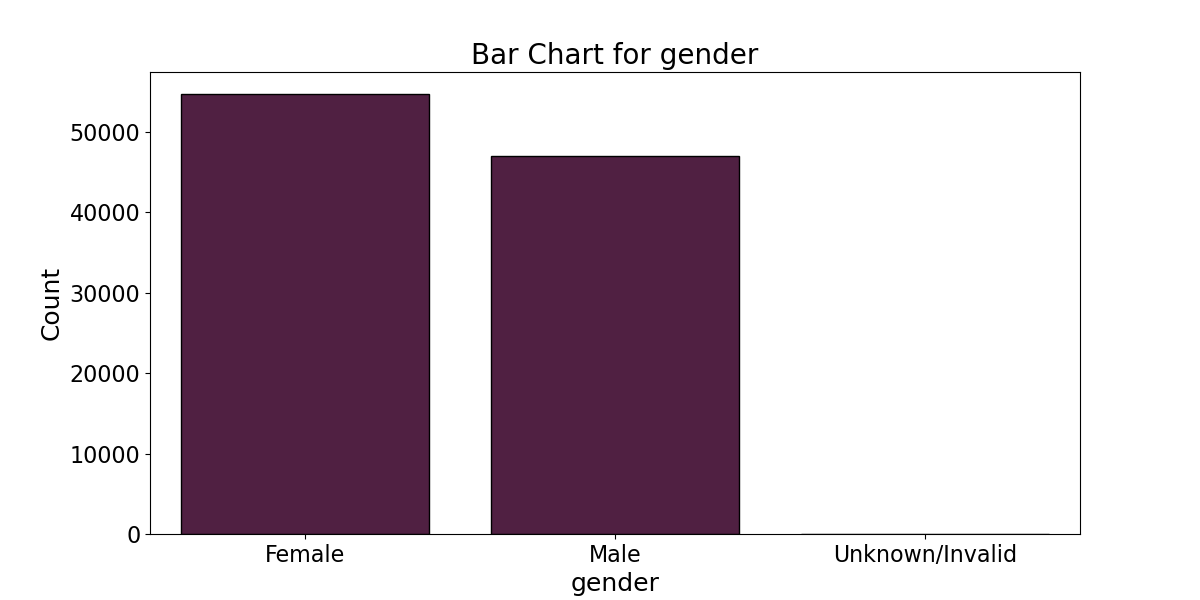
\includegraphics[width=200px]{eda/bar_charts/gender_bar_chart.png}%
\caption{Bar Chart of gender}%
\end{figure}

%


\begin{figure}[h!]%
\centering%
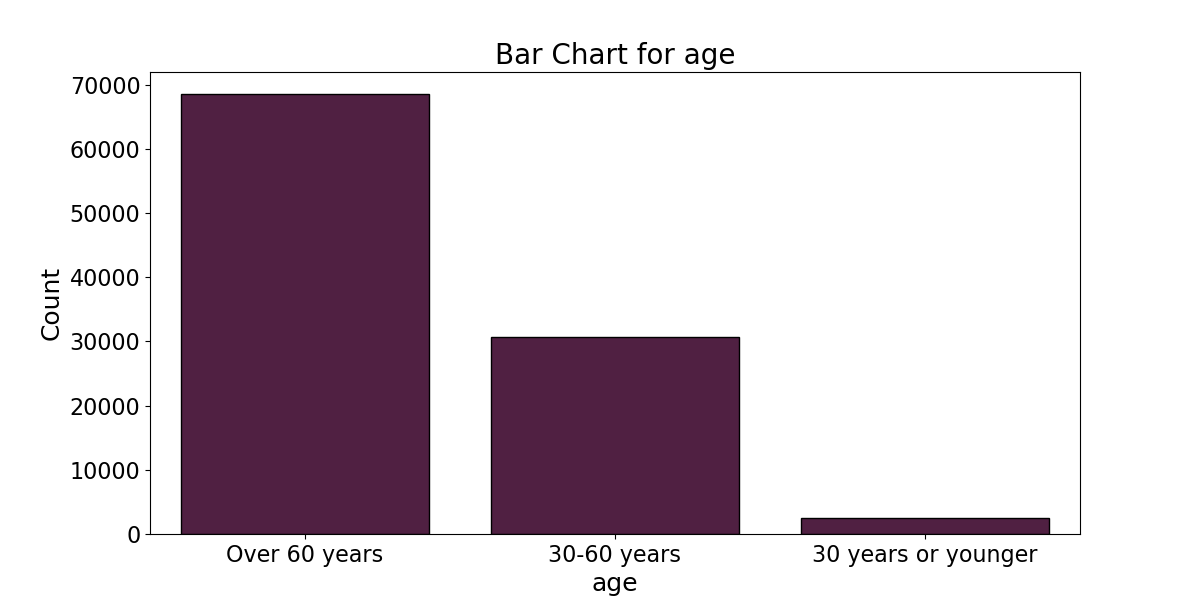
\includegraphics[width=200px]{eda/bar_charts/age_bar_chart.png}%
\caption{Bar Chart of age}%
\end{figure}

%


\begin{figure}[h!]%
\centering%
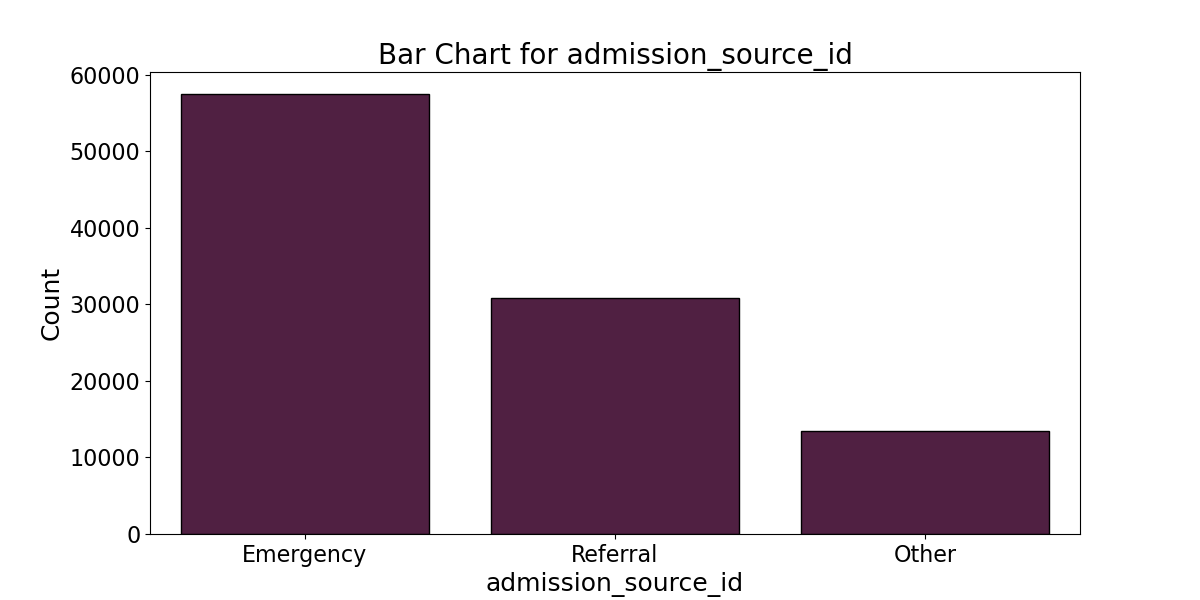
\includegraphics[width=200px]{eda/bar_charts/admission_source_id_bar_chart.png}%
\caption{Bar Chart of admission\_source\_id}%
\end{figure}

%


\begin{figure}[h!]%
\centering%
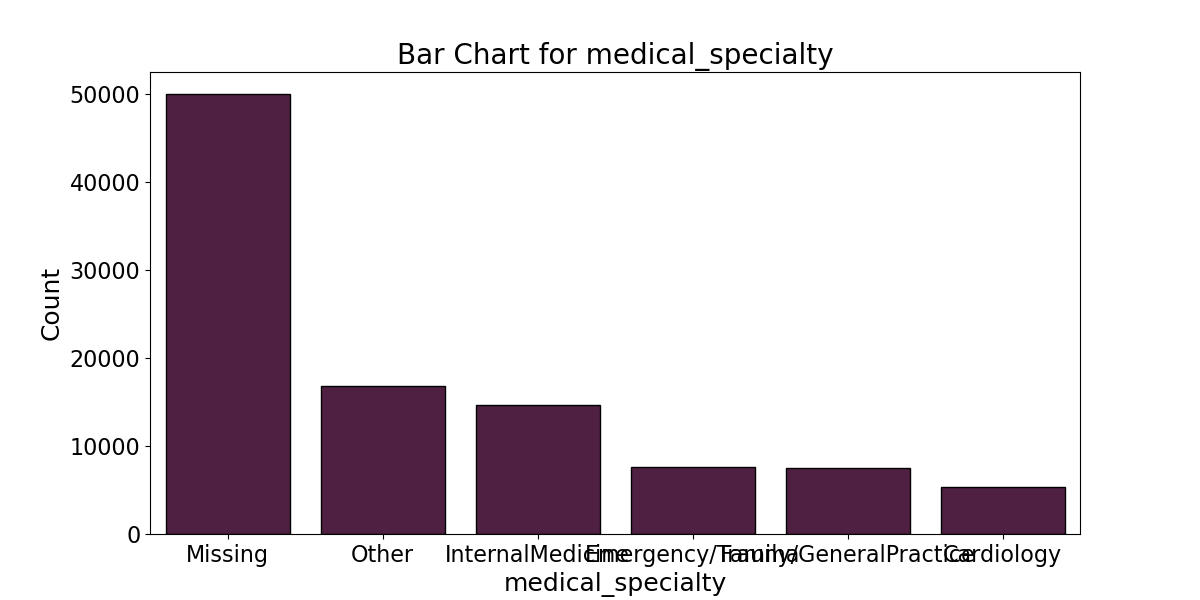
\includegraphics[width=200px]{eda/bar_charts/medical_specialty_bar_chart.png}%
\caption{Bar Chart of medical\_specialty}%
\end{figure}

%


\begin{figure}[h!]%
\centering%
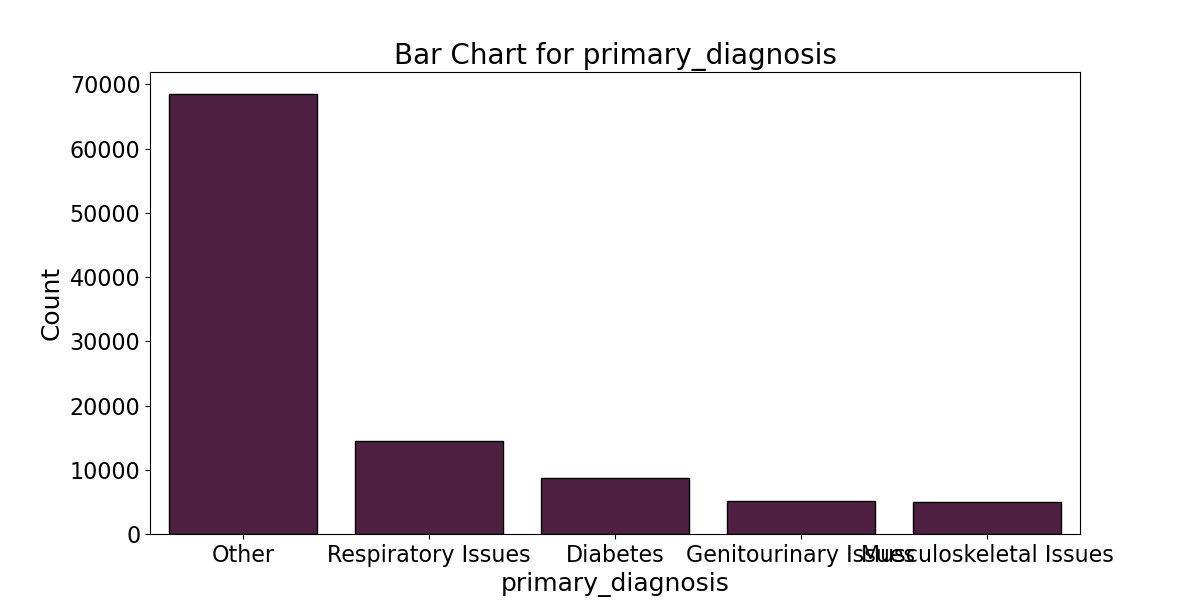
\includegraphics[width=200px]{eda/bar_charts/primary_diagnosis_bar_chart.png}%
\caption{Bar Chart of primary\_diagnosis}%
\end{figure}

%


\begin{figure}[h!]%
\centering%
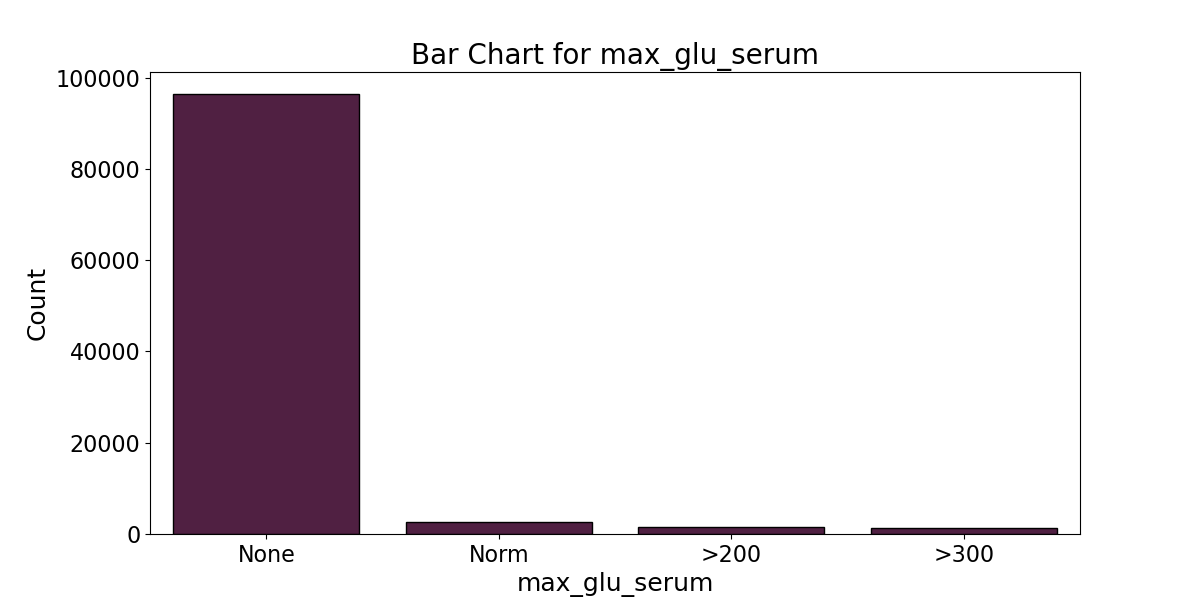
\includegraphics[width=200px]{eda/bar_charts/max_glu_serum_bar_chart.png}%
\caption{Bar Chart of max\_glu\_serum}%
\end{figure}

%


\begin{figure}[h!]%
\centering%
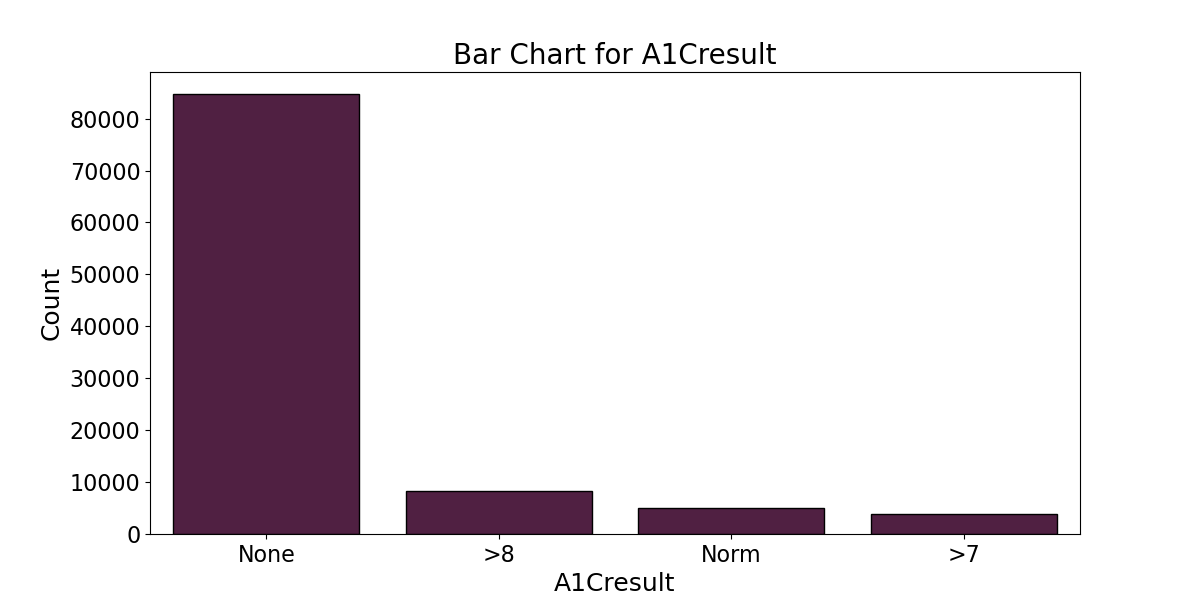
\includegraphics[width=200px]{eda/bar_charts/A1Cresult_bar_chart.png}%
\caption{Bar Chart of A1Cresult}%
\end{figure}

%


\begin{figure}[h!]%
\centering%
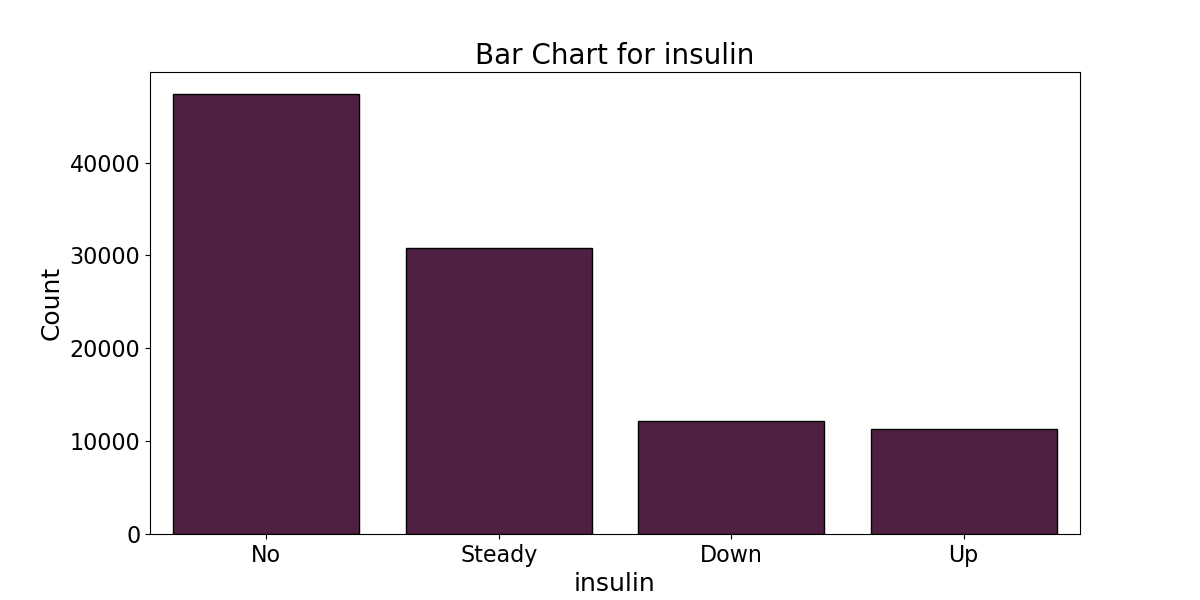
\includegraphics[width=200px]{eda/bar_charts/insulin_bar_chart.png}%
\caption{Bar Chart of insulin}%
\end{figure}

%


\begin{figure}[h!]%
\centering%
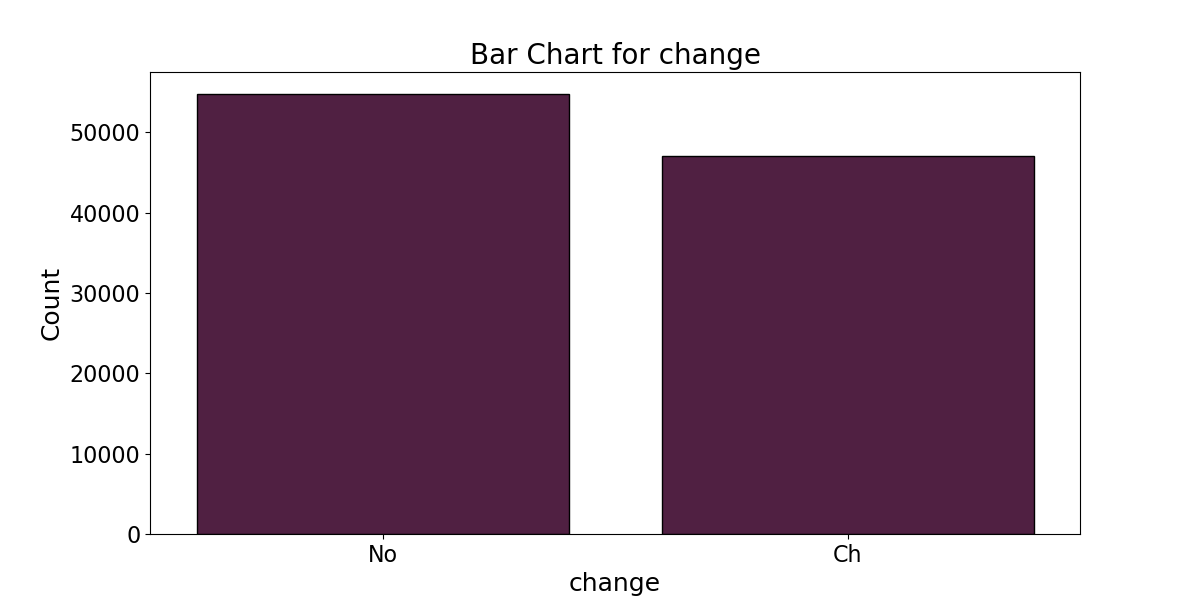
\includegraphics[width=200px]{eda/bar_charts/change_bar_chart.png}%
\caption{Bar Chart of change}%
\end{figure}

%


\begin{figure}[h!]%
\centering%
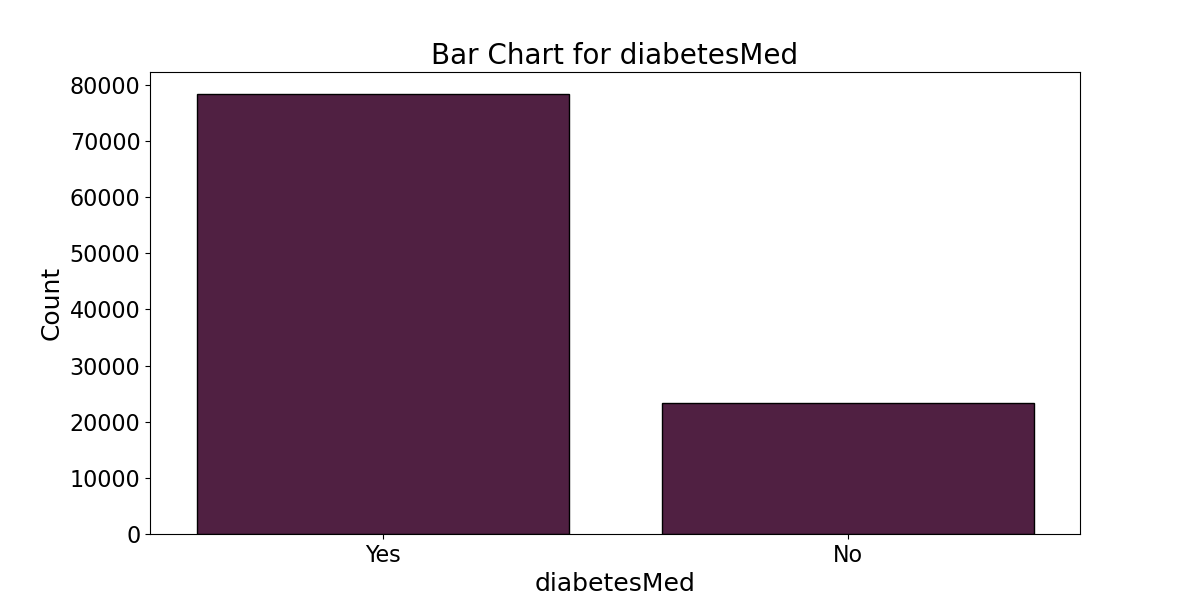
\includegraphics[width=200px]{eda/bar_charts/diabetesMed_bar_chart.png}%
\caption{Bar Chart of diabetesMed}%
\end{figure}

%


\begin{figure}[h!]%
\centering%
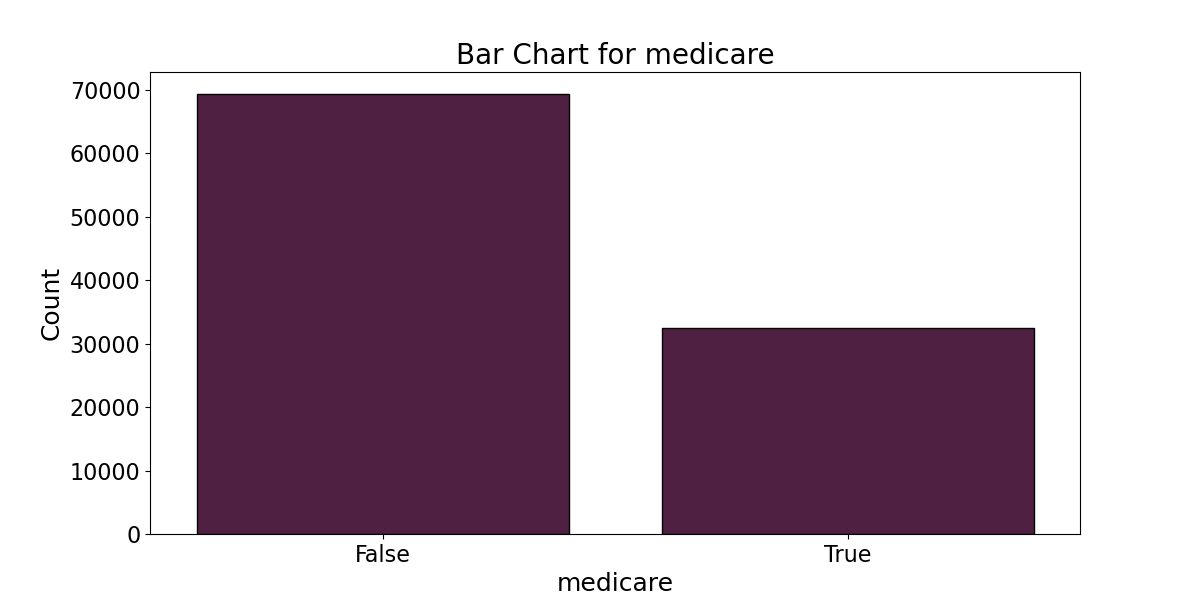
\includegraphics[width=200px]{eda/bar_charts/medicare_bar_chart.png}%
\caption{Bar Chart of medicare}%
\end{figure}

%


\begin{figure}[h!]%
\centering%
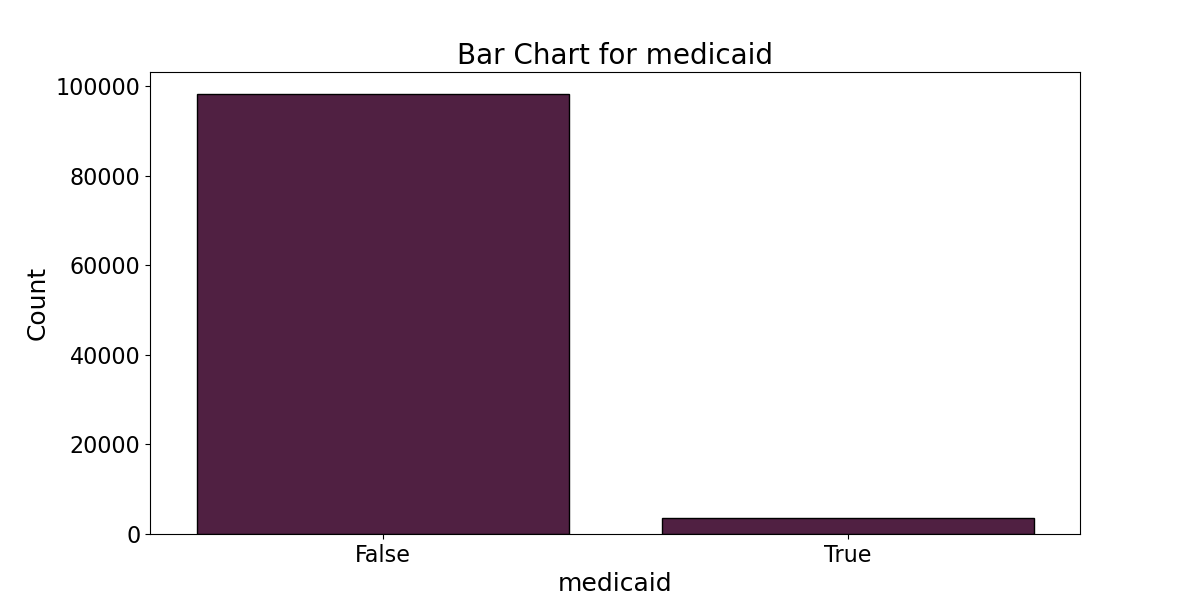
\includegraphics[width=200px]{eda/bar_charts/medicaid_bar_chart.png}%
\caption{Bar Chart of medicaid}%
\end{figure}

%


\begin{figure}[h!]%
\centering%
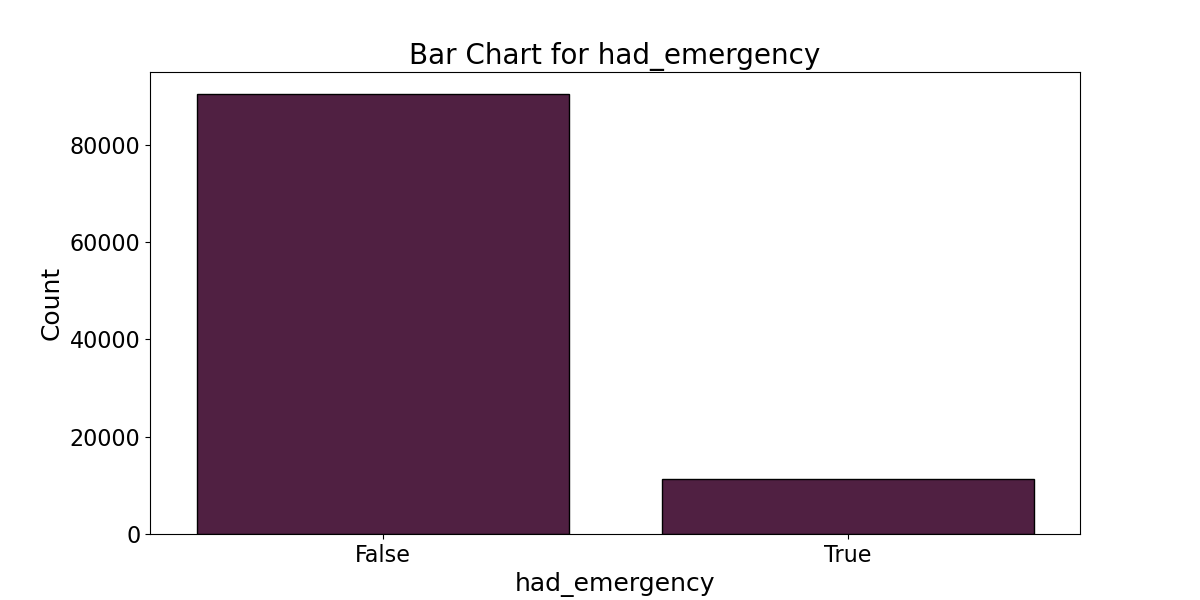
\includegraphics[width=200px]{eda/bar_charts/had_emergency_bar_chart.png}%
\caption{Bar Chart of had\_emergency}%
\end{figure}

%


\begin{figure}[h!]%
\centering%
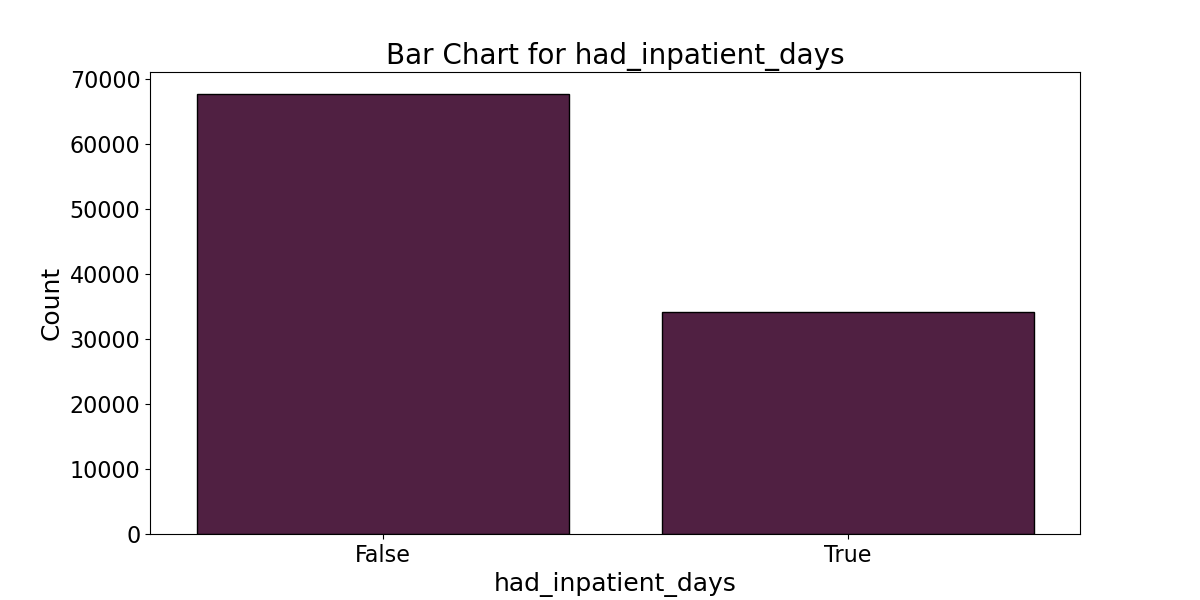
\includegraphics[width=200px]{eda/bar_charts/had_inpatient_days_bar_chart.png}%
\caption{Bar Chart of had\_inpatient\_days}%
\end{figure}

%


\begin{figure}[h!]%
\centering%
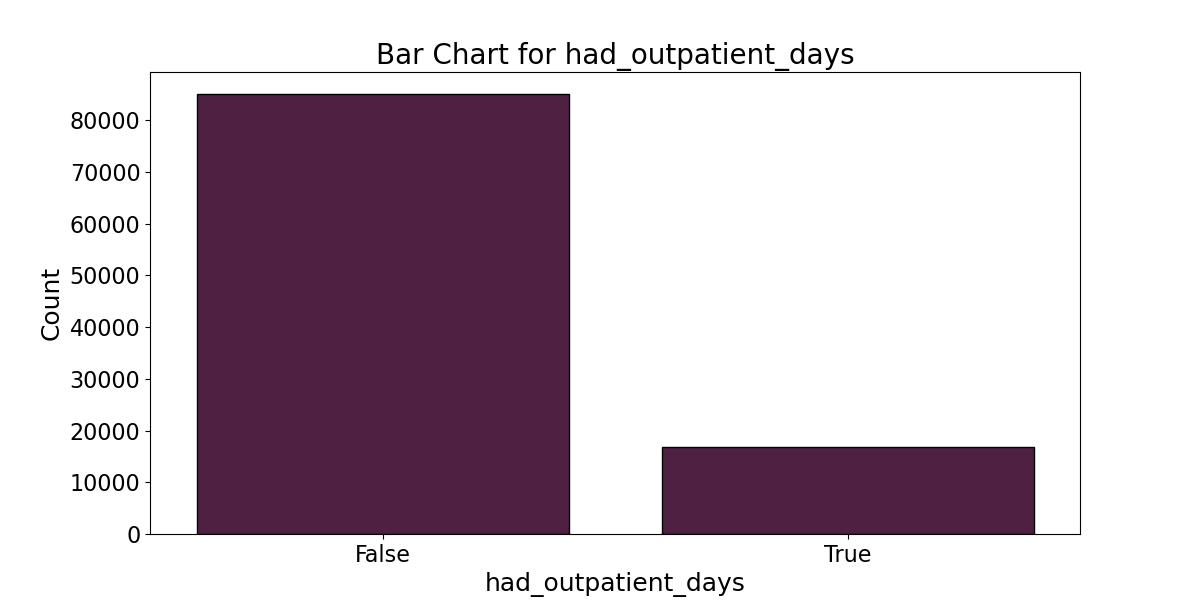
\includegraphics[width=200px]{eda/bar_charts/had_outpatient_days_bar_chart.png}%
\caption{Bar Chart of had\_outpatient\_days}%
\end{figure}

%


\begin{figure}[h!]%
\centering%
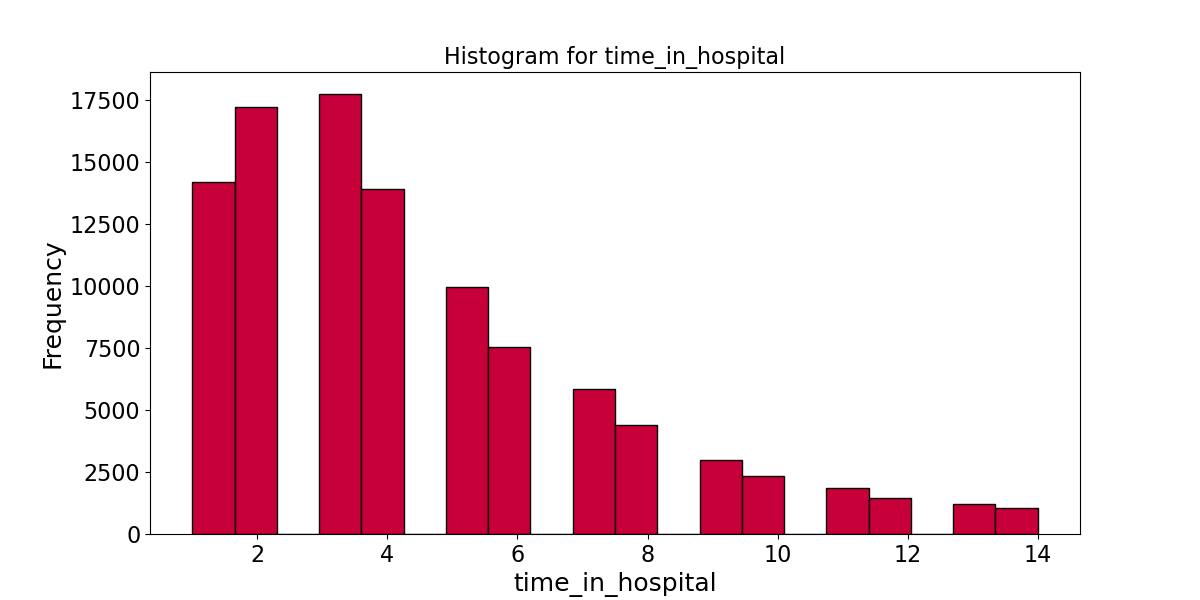
\includegraphics[width=200px]{eda/histograms/time_in_hospital_histogram.png}%
\caption{Histogram of time\_in\_hospital}%
\end{figure}

%


\begin{figure}[h!]%
\centering%
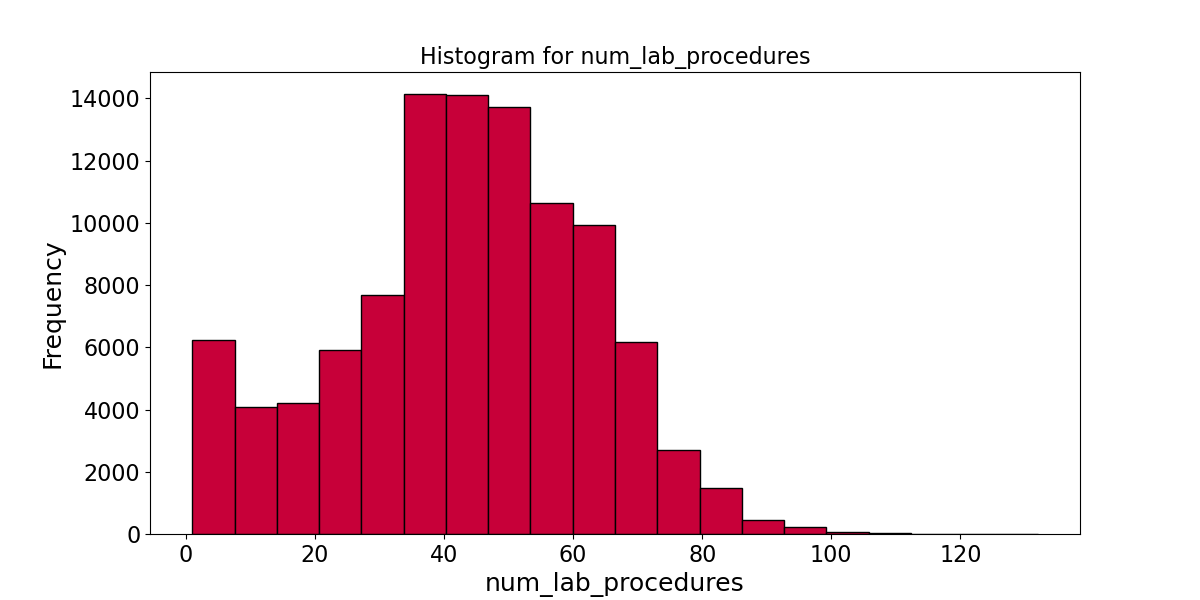
\includegraphics[width=200px]{eda/histograms/num_lab_procedures_histogram.png}%
\caption{Histogram of num\_lab\_procedures}%
\end{figure}

%


\begin{figure}[h!]%
\centering%
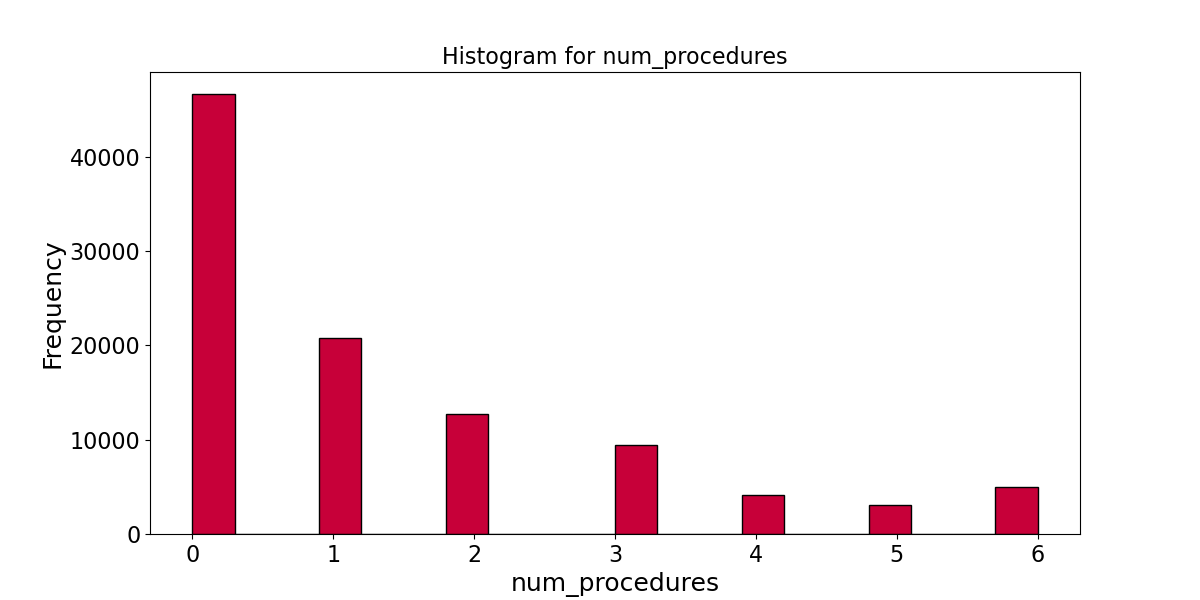
\includegraphics[width=200px]{eda/histograms/num_procedures_histogram.png}%
\caption{Histogram of num\_procedures}%
\end{figure}

%


\begin{figure}[h!]%
\centering%
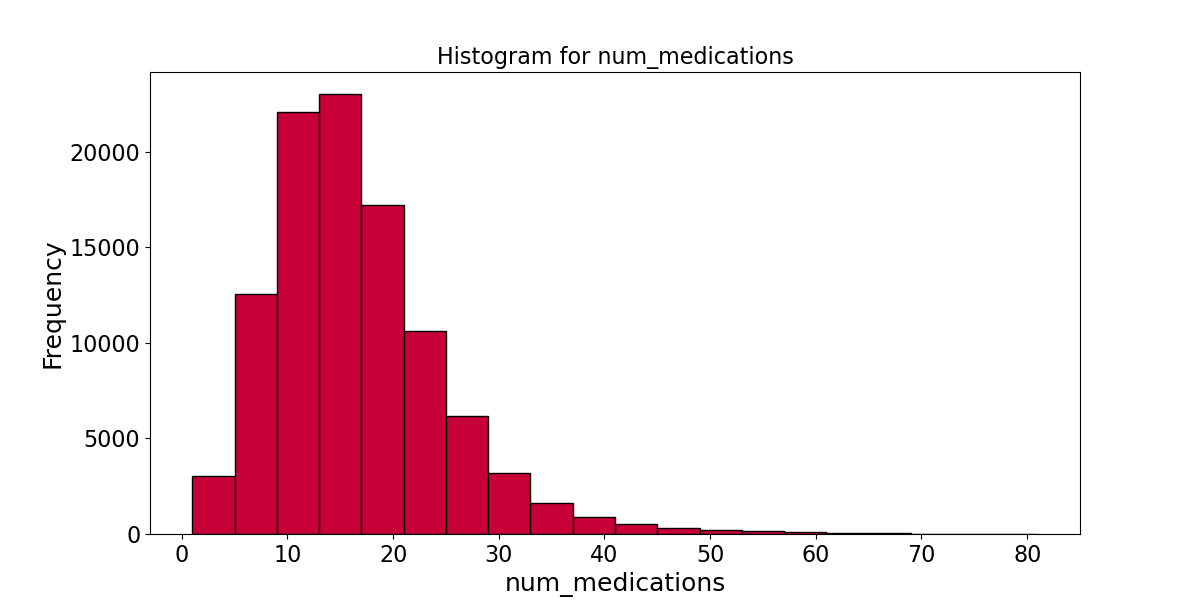
\includegraphics[width=200px]{eda/histograms/num_medications_histogram.png}%
\caption{Histogram of num\_medications}%
\end{figure}

%


\begin{figure}[h!]%
\centering%
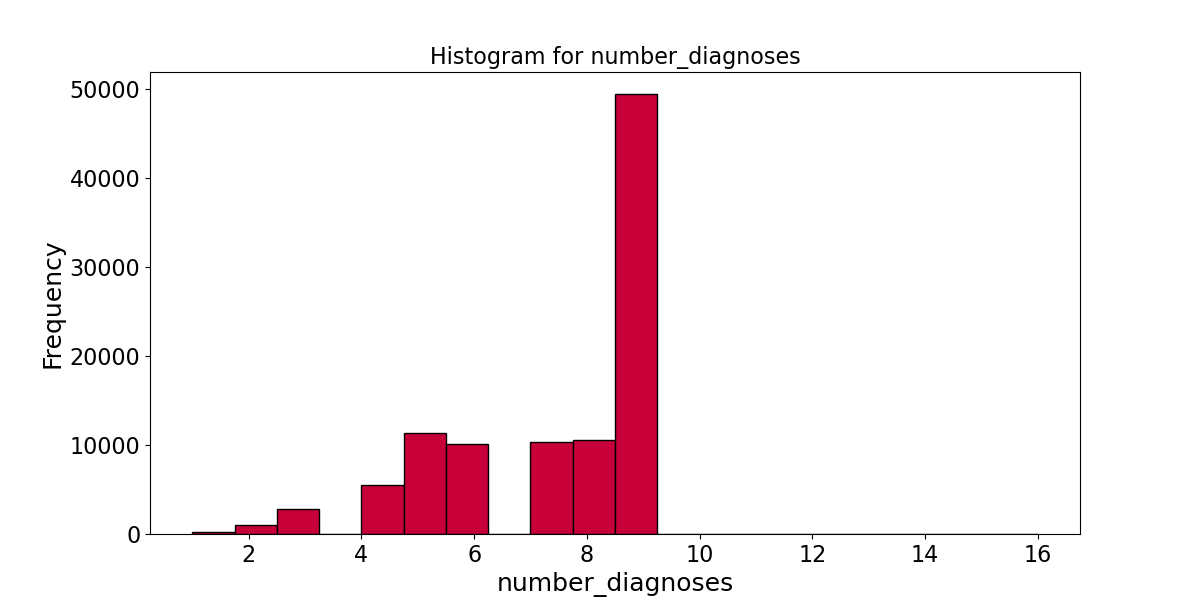
\includegraphics[width=200px]{eda/histograms/number_diagnoses_histogram.png}%
\caption{Histogram of number\_diagnoses}%
\end{figure}

%


\begin{figure}[h!]%
\centering%
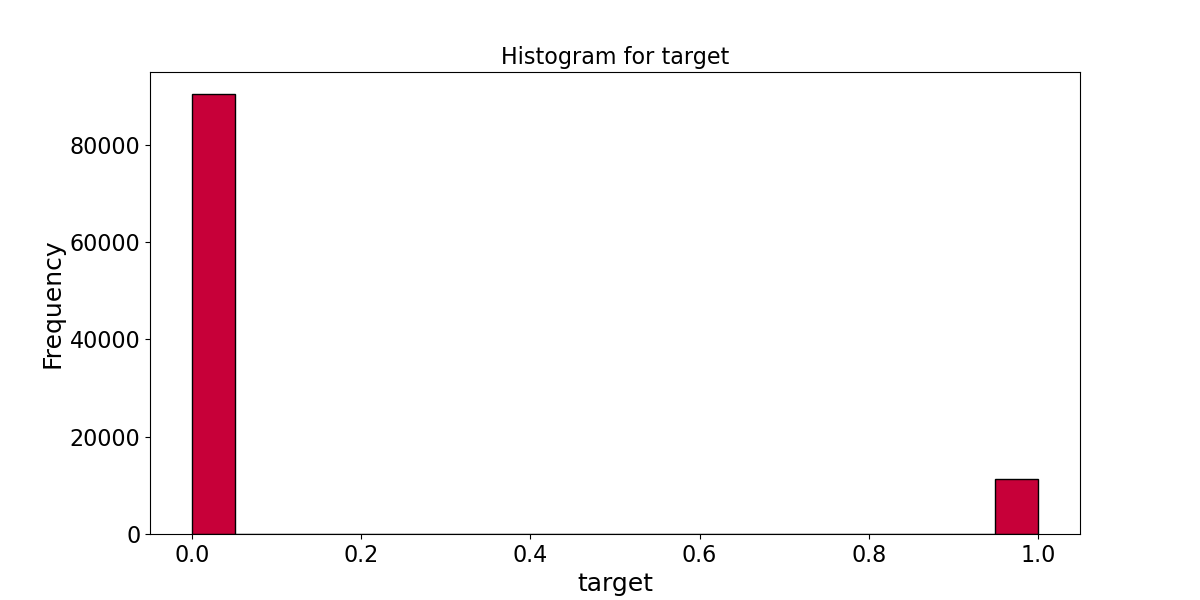
\includegraphics[width=200px]{eda/histograms/target_histogram.png}%
\caption{Histogram of target}%
\end{figure}

%
\end{document}